\subsubsection{Implementation of MIPS processor - Data Path}

Implementing a MIPS processor isn't difficult. On the following page we show three different diagrams: the first is a very high level data path to allow the reader to understand how it works; the second is more detailed, but without the CU (Control Unit); the third is the complete data path and it also includes the CU (in red).

\begin{figure}[!htp]
    \centering
    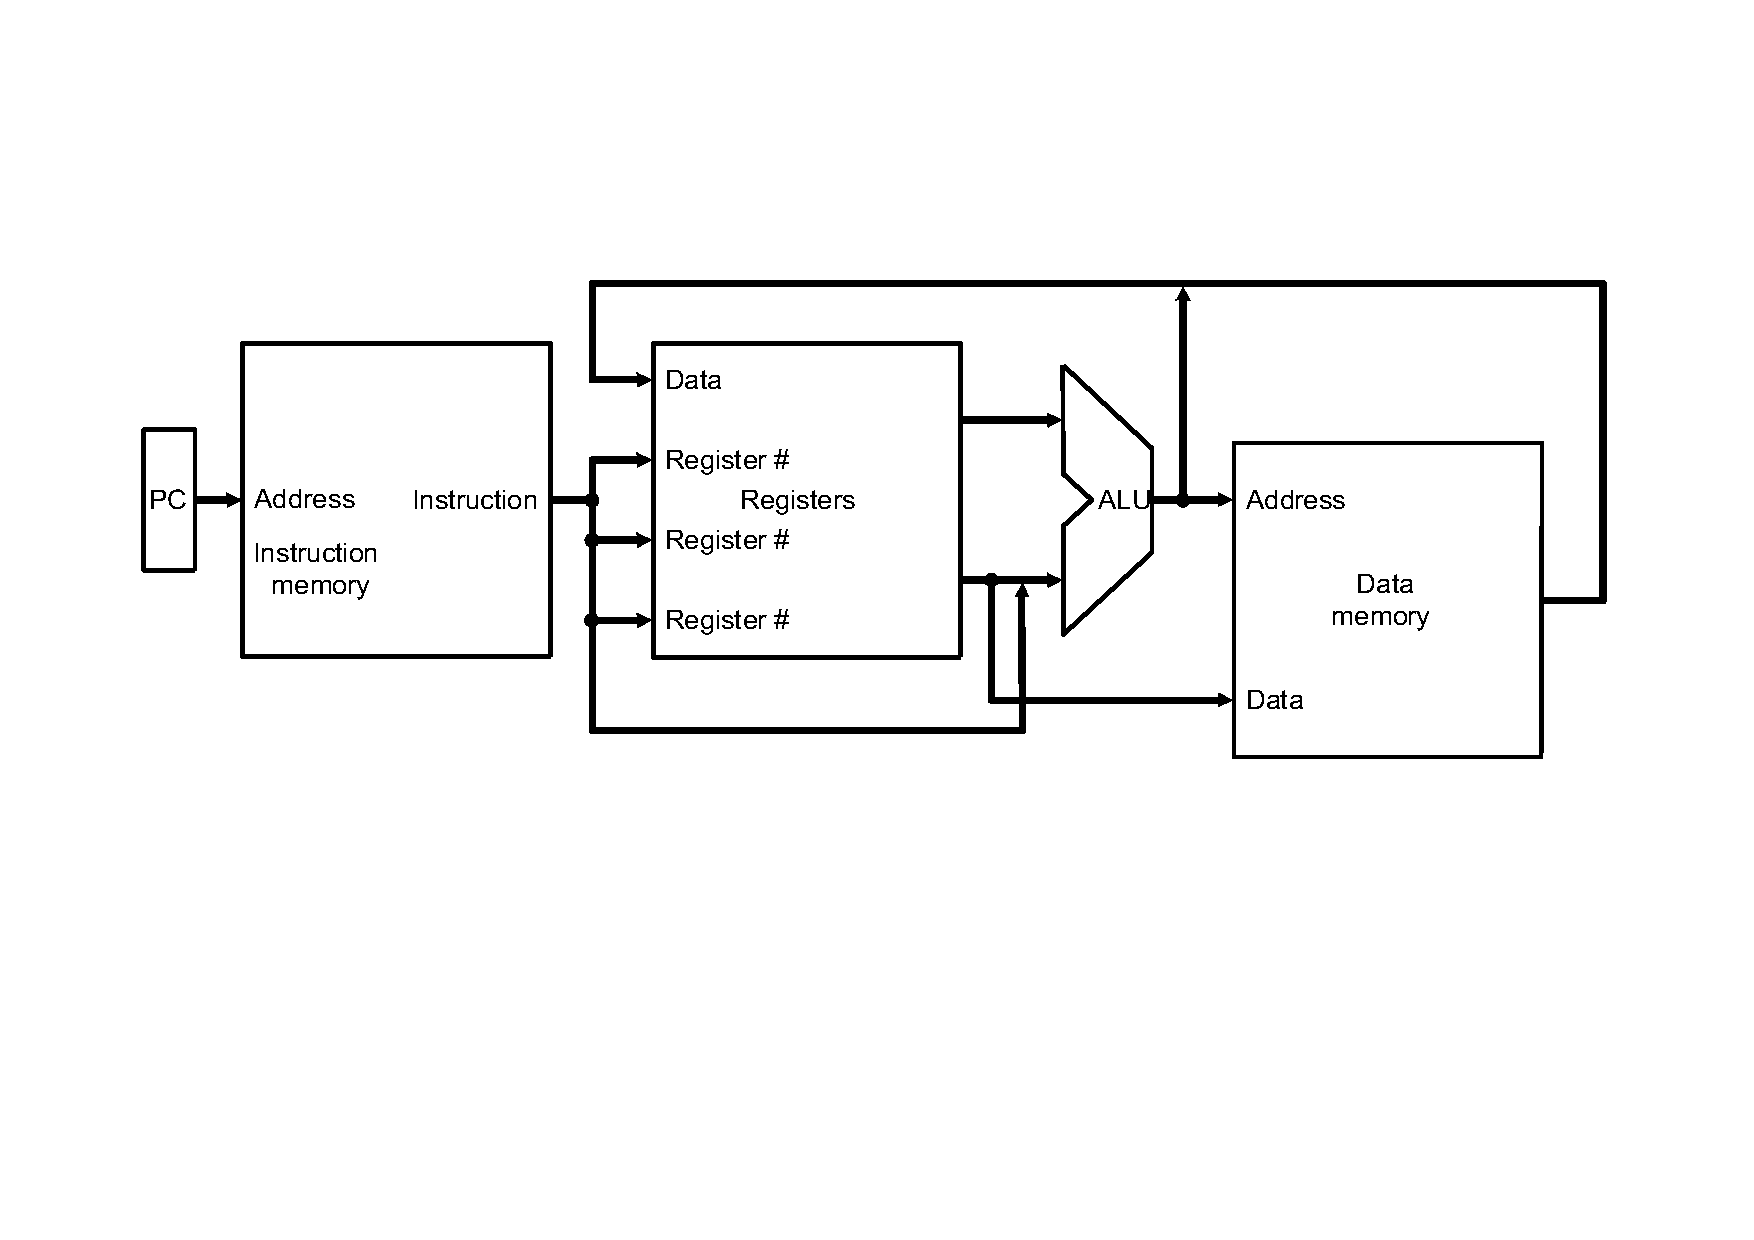
\includegraphics[width=\textwidth]{img/basic-implementation-mips-datapath.pdf}
    \caption{A basic implementation of MIPS data path.\cite{pipelining-slides}}
    \label{fig: basic implementation of MIPS data path}
\end{figure}

\noindent
Scan (or click) the QR code below to view the figure~\ref{fig: basic implementation of MIPS data path} in high quality:
\begin{center}
    \qrcode{https://github.com/PoliMI-HPC-E-notes-projects-AndreVale69/HPC-E-PoliMI-university-notes/tree/main/advanced-computer-architectures/notes/img/basic-implementation-mips-datapath.pdf}
\end{center}
Two notes:
\begin{itemize}
    \item The \textbf{Instruction Memory} (read-only memory) is separated from \textbf{Data Memory}.
    
    \item The 32 general-purpose register are organized in a \textbf{Register File} (RF) with 2 read ports and 1 write port.
\end{itemize}

\begin{figure}[!htp]
    \centering
    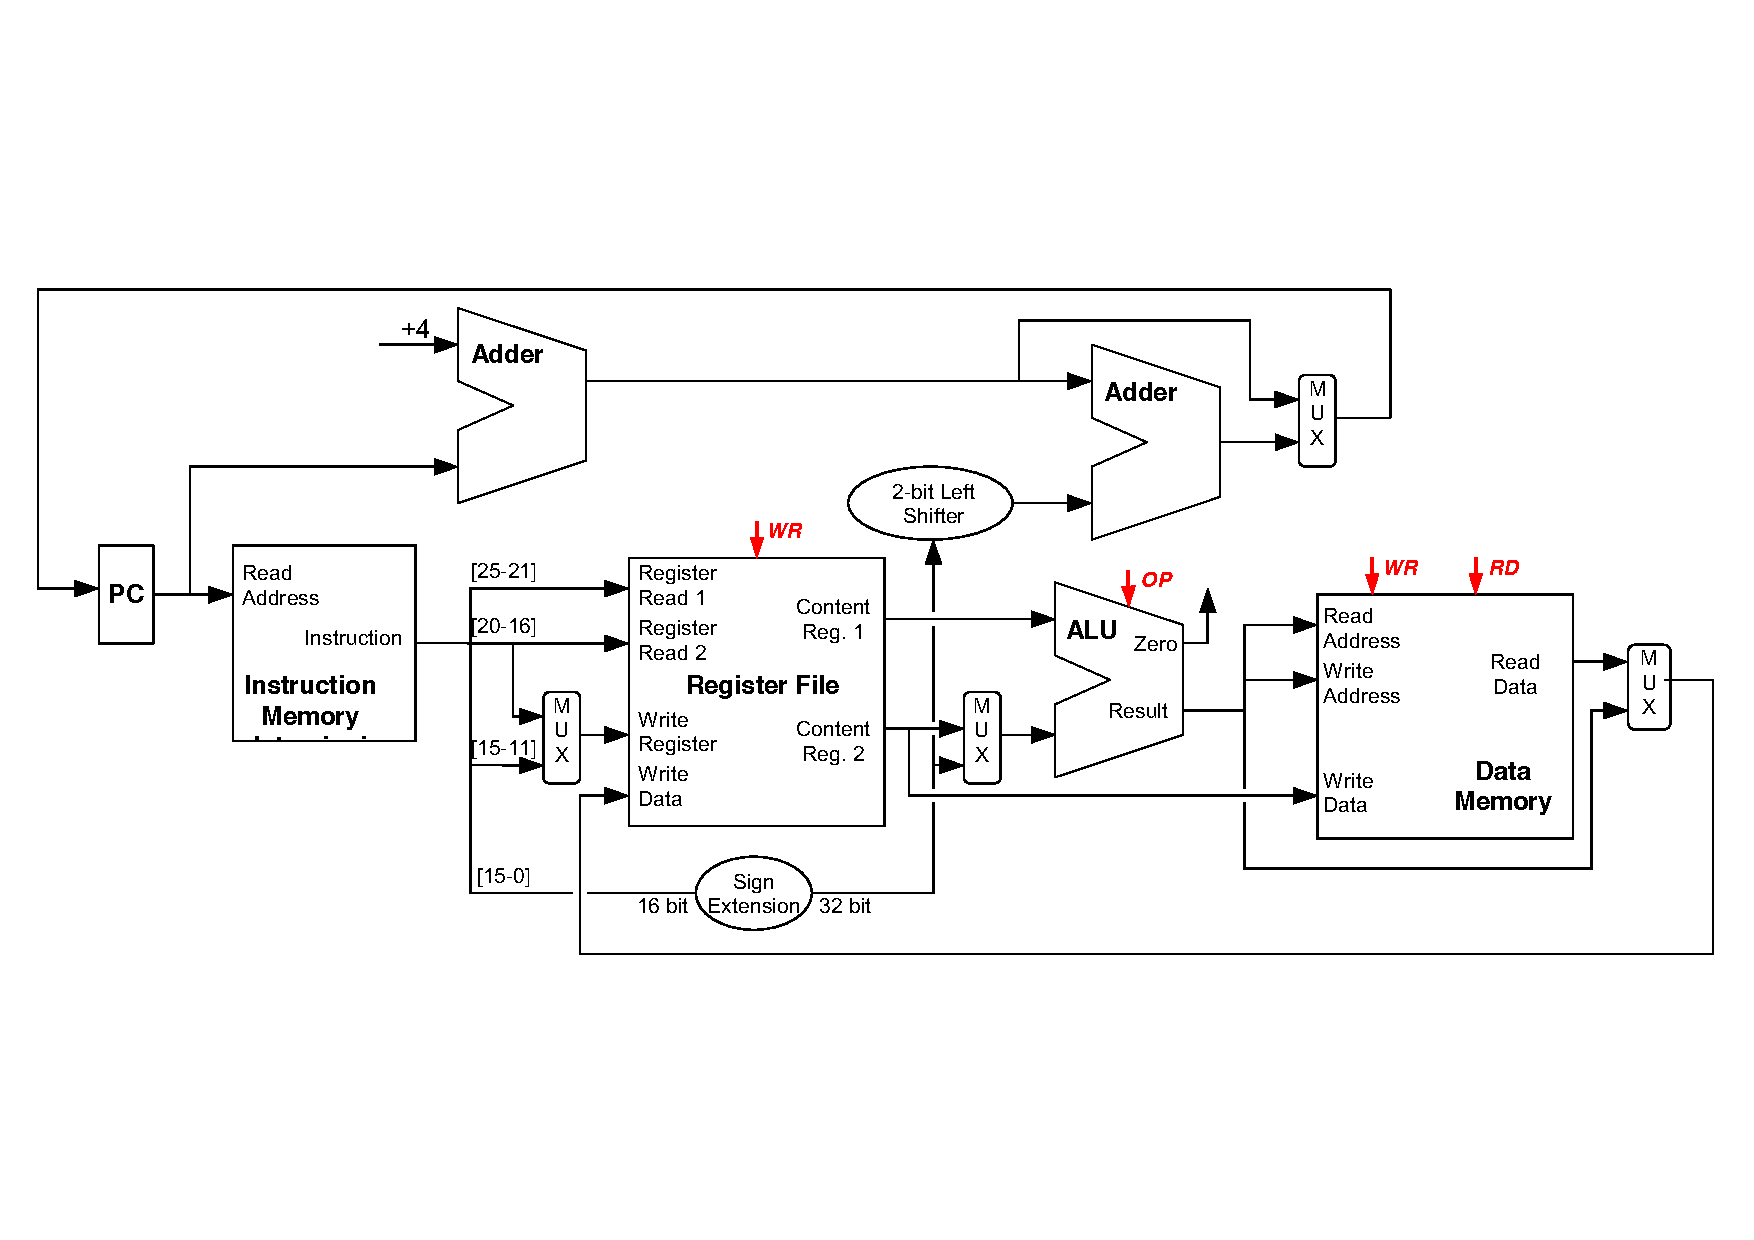
\includegraphics[width=\textwidth]{img/implementation-mips-datapath.pdf}
    \caption{An implementation of MIPS data path (no Control Unit).\cite{pipelining-slides}}
    \label{fig: implementation of MIPS data path (no Control Unit)}
\end{figure}

\newpage

\noindent
Scan (or click) the QR code below to view the figure~\ref{fig: implementation of MIPS data path (no Control Unit)} in high quality:
\begin{center}
    \qrcode{https://github.com/PoliMI-HPC-E-notes-projects-AndreVale69/HPC-E-PoliMI-university-notes/tree/main/advanced-computer-architectures/notes/img/implementation-mips-datapath.pdf}
\end{center}

\begin{figure}[!htp]
    \centering
    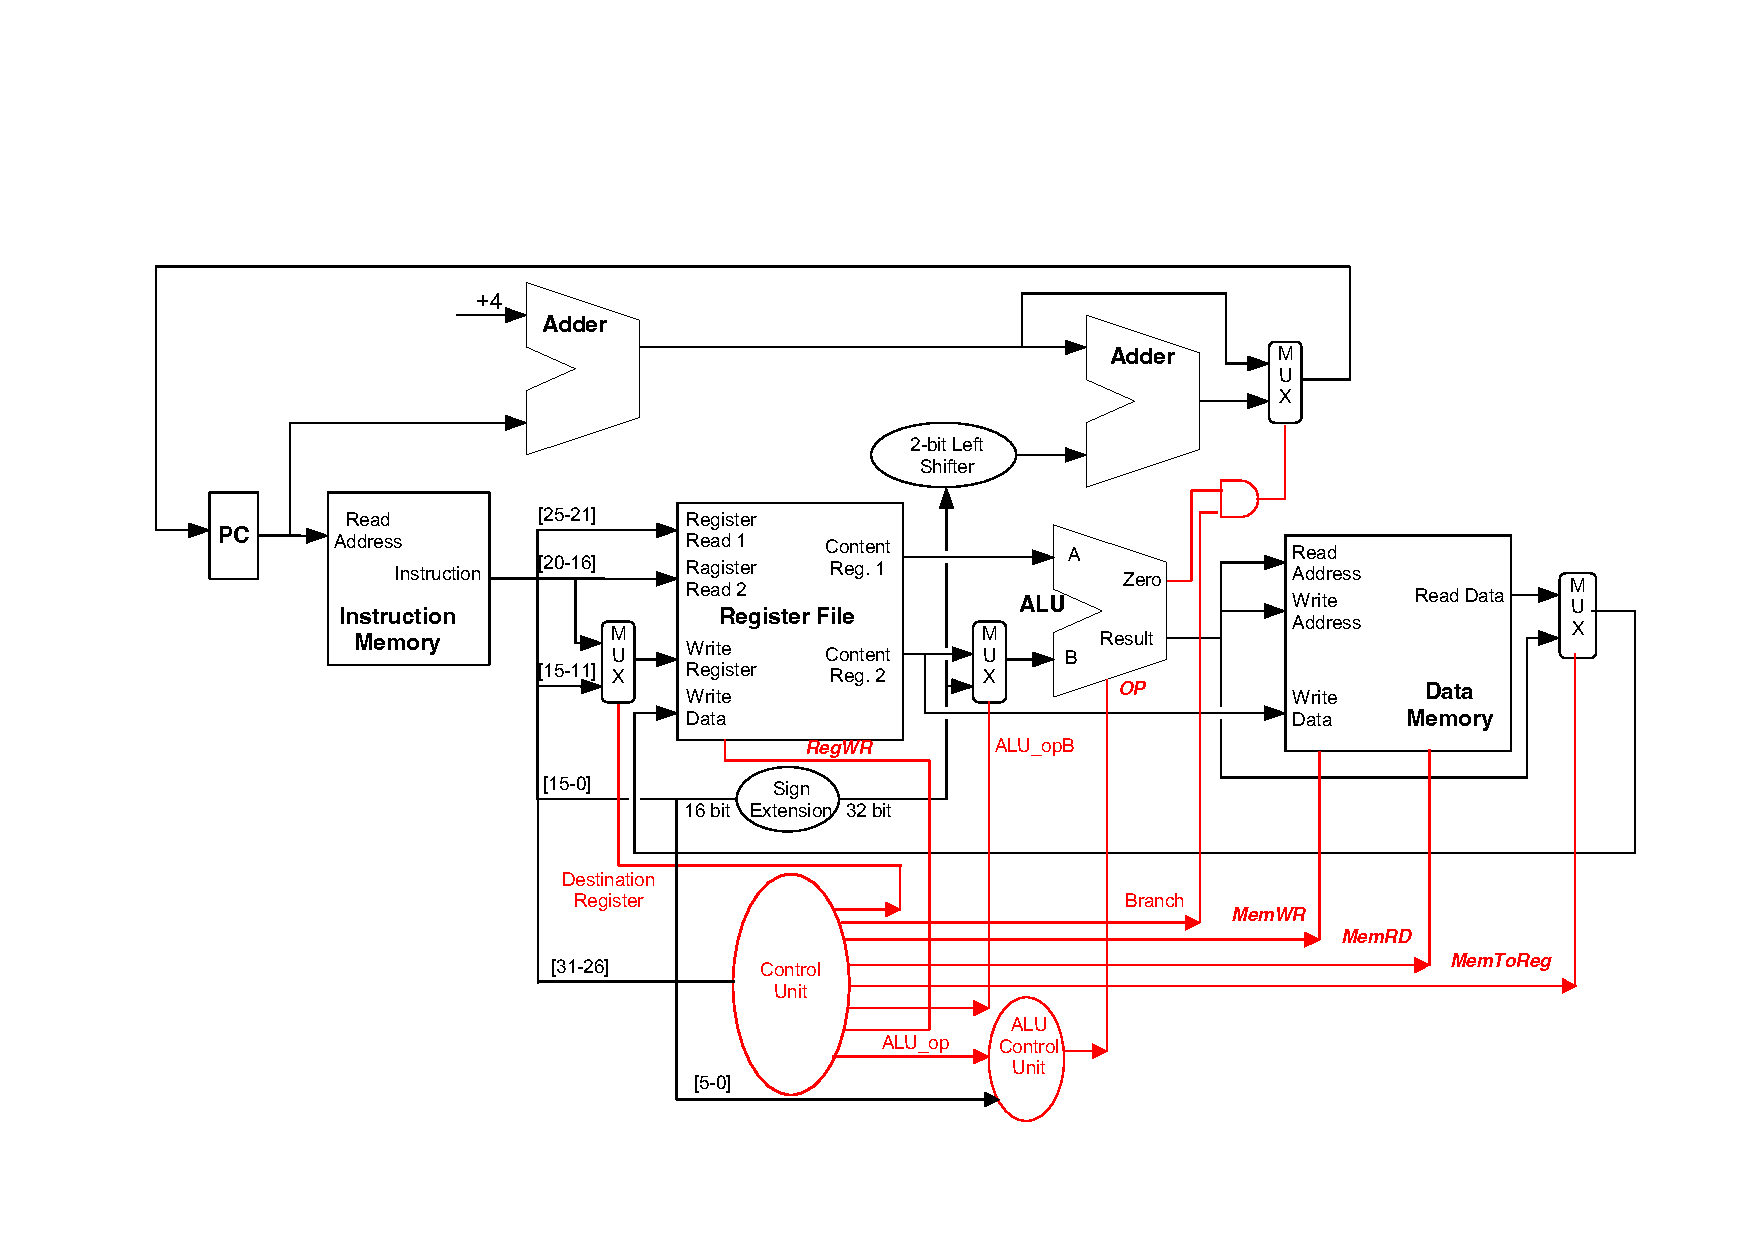
\includegraphics[width=\textwidth]{img/implementation-mips-datapath-cu.pdf}
    \caption{A complete implementation of MIPS data path.\cite{pipelining-slides}}
    \label{fig: complete implementation of MIPS data path}
\end{figure}

\noindent
Scan (or click) the QR code below to view the figure~\ref{fig: complete implementation of MIPS data path} in high quality:
\begin{center}
    \qrcode{https://github.com/PoliMI-HPC-E-notes-projects-AndreVale69/HPC-E-PoliMI-university-notes/tree/main/advanced-computer-architectures/notes/img/implementation-mips-datapath-cu.pdf}
\end{center}